% Created 2019-06-02 dom 19:18
% Intended LaTeX compiler: pdflatex
\documentclass[a4paper,12pt,oneside]{article}
\usepackage[main=spanish, english, ]{babel}%paquete para el idioma del documento. Si
%se quiere utilizar un parrafo con idioma diferente podemos utilizar
%la orden  electlanguage{}
\usepackage[utf8]{inputenx}
\usepackage[T1]{fontenc}
\usepackage{lmodern,pifont}
\usepackage{pdflscape}
\usepackage{caption}
\usepackage{textcomp}
\usepackage{graphicx}
\usepackage[dvipsnames]{color}
\usepackage{colortbl}
\usepackage{longtable}
\usepackage{hyperref}
\hypersetup{bookmarksopen,bookmarksnumbered,bookmarksopenlevel=4,%
  linktocpage,colorlinks,urlcolor=black,citecolor=ForestGreen,linkcolor=black,filecolor=black}
\usepackage{natbib}
\usepackage{amssymb}
\usepackage{amsmath}
\usepackage{geometry}
\geometry{a4paper,left=2cm,top=2cm,right=2.5cm,bottom=2cm,marginparsep=7pt, marginparwidth=.6in}
\usepackage[utf8]{inputenc}
\usepackage[T1]{fontenc}
\usepackage{graphicx}
\usepackage{grffile}
\usepackage{longtable}
\usepackage{wrapfig}
\usepackage{rotating}
\usepackage[normalem]{ulem}
\usepackage{amsmath}
\usepackage{textcomp}
\usepackage{amssymb}
\usepackage{capt-of}
\usepackage{hyperref}
\author{Antonio Soler Gelde. IT Forestal}
\date{}
\title{UF1597. Manejo de instalaciones y expedición de plantas en vivero.}
\hypersetup{
 pdfauthor={Antonio Soler Gelde. IT Forestal},
 pdftitle={UF1597. Manejo de instalaciones y expedición de plantas en vivero.},
 pdfkeywords={},
 pdfsubject={},
 pdfcreator={Emacs 25.3.1 (Org mode 8.2.10)}, 
 pdflang={Spanish}}
\begin{document}

\maketitle
\thispagestyle{empty} \tableofcontents \clearpage\section{Medio de cultivo para plantas de vivero}
\label{sec:org71fdd03}
\subsection{Introducción}
\label{sec:org0ae2db9}
El sustrato en el que cultivamos las plantas y/o hortalizas en el viviero es muy
importante. Propiedades como la textura, drenaje y disponibilidad de nutrientes
han de promover el crecimiento de las plantulas y ademas facilitar su extracción
para poder sacar el cepellón sin que este se rompa.
\subsection{Componentes para la elaboración del medio de cultivo de plantas en vivero}
\label{sec:org949e834}
\subsubsection{Sustratos}
\label{sec:orgc793a50}
Para la producción de plantas ornamentales el sustrato se emplea como soporte y
alimento y va a ser la base sobre la que se va a desarrollar. Por ello es muy
importante entender que el futuro de la produccion va a depender mucho del tipo
de sustrato sobre el que se inicia el cultivo. 
\subsubsection{Características de un buen susutrato}
\label{sec:org89d77ec}
\begin{itemize}
\item Estabilidad física: Qué mantenga sus características fisicas durante un
tiempo razonable
\item Baja densidad
\item Aireación
\item pH adecuado al tipo de planta
\item Esterilidad: libre de patogenos que puedan dañar la planta o de semillas que
puedan crear una competencia no deseada
\item Fertilidad
\item Capacidad de retención de nutrientes
\item Capacidad de retención de agua
\end{itemize}
\subsubsection{Materiales utilizados en la preparación de sustratos}
\label{sec:orge3dcef5}
Existe una gran variedad,y  pueden ser tanto de origen orgánico e inorgánico:
\begin{itemize}
\item Turba rubia y turba negra
\item Fibra de coco
\item Restos de poda y residuos de jardineria triturados
\item Lodos de depuradoras
\item Residuos forestales
\item Arenas, gravas
\item Materiales sintéticos: perlita, vermiculita, lana de roca, poliestireno, etc
\end{itemize}
El empleo de tierras y mantillos así como de estiercol \textbf{está restringido} porque
pueden estar contaminadas con semillas de especies no deseadas y/o
enfermedades.\\
A la hora de elaborar un sustrato hay que conocer su \textbf{destino y
particularidades}:\\
\begin{itemize}
\item \textbf{Producción viverista:} Para plantas de interior y exterior. Formados
principalmente por turba y fibra de coco.
\item \textbf{Multiplicación de plantas:} Pueden ser para \uline{semilleros}, \uline{esquejes}, o
producción de planta forestal. Se suelen hacer con mezclas de turba rubia y negra
\item \textbf{Hidroponía:} Un tipo de producción muy especial. En este caso los sustratos
empleados pueden ser inertes ya que todos los nutrientes se aplican a traves
del agua de riego. Suelen estar compuestos de perlita, vermiculita, lana de
roca o fibra de coco.
\end{itemize}
\subsection{Características de los sustratos}
\label{sec:org1394c37}
\subsubsection{Características físicas}
\label{sec:org9e53e54}
\begin{itemize}
\item \textbf{Textura:} La proporción de arena, limo y arcilla en los suelos determina el
tipo de textura que un suelo tiene. La textura va a determinar propiedades
como la capacidad de retención de agua y está relacionada directamente con
otras propiedades como la porosidad, densidad y estructura.
\item \textbf{Porosidad:}
\end{itemize}
La porosidad de un sustrato es el vlumen que no está siendo ocupado por
particulas solidas, minerales u orgánicas. Estos espacios no ocupados se llenan
de agua o aire.
La proporción de estos espacios no debe ser inferior al 80-85\%.\\
\begin{center}
\begin{figure}[htbp]
\centering
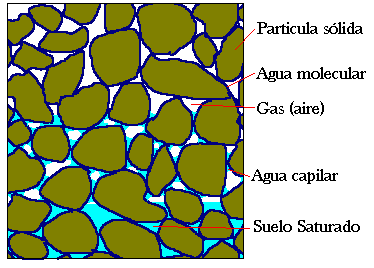
\includegraphics[width=.9\linewidth]{/img_uf1596/porosidad.PNG}
\caption{\label{fig:org977db36}
Porosidad en suelos}
\end{figure}
\end{center}
El grosor de los poros condiciona la aireación y retención de agua. Los porors
en el suelo se distiguen en \textbf{macroscópicos} y \textbf{microscópicos}.\\
Los terrenos \textbf{arenosos} tienen gran cantidad de poros macroscópicos por lo que tienen una 
muy baja capacidad de retención e agua. Por otro lado los suelos \textbf{arcillosos}
son son ricos en poros microscópicos por lo que tienen una gran capacidad de
retención de agua.
\begin{itemize}
\item \textbf{Densidad:}
\end{itemize}
La relación entre la masa de un suelo y el volumen aparente que ocupa, que
incluye el volumen que ocupan los poros, se denomina densidad aparente.\\
 Es una característica importante de los suelos, puesto que permite conocer su
comportamiento hídrico (capacidad de almacenaje de agua, permeabilidad, etc.) y
sobre su función como hábitat (compactación, facilidad para la penetración de
las ra´ıces, apertura de galerías, etc.), entre otras.
\begin{itemize}
\item \textbf{Estructura:}
\end{itemize}
La estructura de un suelo es la manera en la que están dispuestos sus
componentes. Las partículas de arena, limo y arcilla se unen entre si de
determinadas maneras formando \uline{terrones}. Según como se unen las partículas y la
forma que adquieren se clasifican en:
\begin{itemize}
\item \textbf{De grano simple:} Frecuente en suelos arenososo ya que los granos
de arena no se unen entre si y se disgregan facilmente
\item \textbf{Granular:} Frecuente en suelos que ya han sido cultivados. Terrones no muy
grandes y redondeados
\item \textbf{De bloques:} Terrones cuadrados y algo más grandes que la granular
\item \textbf{Prismatica:} Terrones más gruesos y alargados
\item \textbf{Laminar:} Muy fácil de identificar por que el suelo está formado por laminas
delgadas horizontales
\item \textbf{Masiva:} En este caso no se forman terrones y el suelo se observa
compacto. Muy común en suelos arcillososo que no han sido cultivados
\end{itemize}
\begin{center}
\begin{figure}[htbp]
\centering
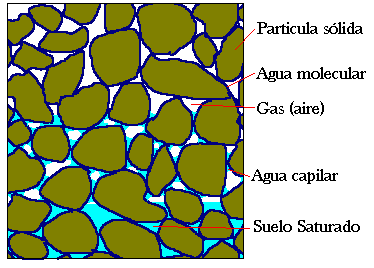
\includegraphics[width=.9\linewidth]{/img_uf1596/porosidad.PNG}
\caption{Principales estructuras en los suelos}
\end{figure}
\end{center}
\subsubsection{Características químicas}
\label{sec:orgc1fdc22}
\subsubsection{Características biológicas}
\label{sec:orgb7259bc}
\subsection{Preparación del medio de cultivo}
\label{sec:orgba50308}
En un viviero además de cultivar plantas en macetas, podemos hacerlo en el
suelo, ya sea dentro de los invernaderos o al aire libre. Un factor \uline{fundamental}
para el desarrollo de las plantas son las \uline{condiciones} del suelo, que se mejoran
entre otras tecnicas mediante el \uline{laboreo}.
La producción y desarrollo de las plantas está ligada a la \uline{porosidad} del
suelo, ya que son sensibles a la aireación y humedad de su sistema radicular. Es
por lo que el laboreo debe ir dirigido, entre otras cosas, a conseguir una buena
\uline{aireación}, es decir, mejorar la porosidad.
\subsection{Realización de mezclas}
\label{sec:org79a5b48}
En los viveros se producen muchos cultivos en contenedor. Esta manera de
producir plantas tiene unas limitaciones que vinen dadas por el tamaño del
contenedor. El \uline{volumen reducido} de sustrato que hay en un contenedor obliga a
\uline{intensificar el riego}, en comparación con un suelo natural en el que las
plantas pueden desarrollar sus raices todo lo necesario para buscar agua. Por
tanto los sustratos tendran como \uline{principal característica} tener una buena
capacidad de \textbf{retención de agua}, pero sin que ello afecte a la \textbf{porosidad} y la
\textbf{densidad}, que como sabemos son factores importantes para el desarrollo de las
raices y de la planta.
\uline{No se recomienda} el uso de suelo mineral como un componente de sustratos para
macetas, aunque en ciertas circunstancias pueda dar buenos resultados, este tipo
de material tiende a disminuir la porosidad del suelo.
Debe utilizarse una cantidad suficiente de \textbf{componentes orgánicos} en los
sustratos. Este debe haber pasado por un proceso de \textbf{compostaje} para que sea
estable, de esta manera la materia organica no se descompondrá mediante
microorganismos que tomarán el nitrogeno del sustrato no dejandolo disponible
para las plantas.
\subsection{Enmiendas y fertilización}
\label{sec:org6013e54}
La mayoría de los componentes orgánicos de un sustrato sn ácidos y contienen
\uline{niveles bajos de nutrientes disponibles}. Se recomienda:
\begin{itemize}
\item Aporte de \textbf{cal}: Elevará el pH y además aportará calcio y magnesio que son
\uline{esenciales para el desarrollo radicular}. Estos elemntos son retenidos por el
sustrato por lo que no se lavan fácilmente.
\item Para asegurar un buen comienzo del cultivo el nitrógeno (N) debe ser incorporado
antes de plantar. Sin embargo esta práctica es \uline{muy discutible} cuando se usan
fertilizantes inorgánicos (tipo \emph{nitrofoska}) debido al efecto de
contaminación que la \uline{sobre-fertilización} produce en los acuiferos.
\item Fósforo (P) y potásio (K) suelen incorporarse junto al nitrógeno en formulas
N-P-K. El fósforo se \uline{lava menos} mientras que el potasio debería ser
\uline{repuesto periodicamente} ya que no es adsorbido fuertemente por el sustrato.
\item En los suelos calcareos el hierro (Fe) no esta facilmente disponible por la
planta debido al pH. La manera más eficiente de aportar este elemento es
mediante \uline{quelato de hierro}, que puede ser adsorbida por la planta en un
rango más amplio de pH.
\end{itemize}
\subsection{Desinfección y otros}
\label{sec:org297cc02}
Los sustratos pueden estar "contaminados" entre otras cosas de:
\begin{itemize}
\item Semillas de malezas y otras hierbas competidoras
\item Bulbos o rizomas de pastos
\item Larvas de insectos
\item Caracoles o babosas
\item Hóngos y patógenos
\item Nemátodos
\end{itemize}
Es muy importante que los sustratos estén debidamente desinfectados. Mencionamos
algunas medidas:
\begin{itemize}
\item \textbf{Cribar} el sustrato para retener partículas grandes de vegetales, insectos u
otros organismos
\item \textbf{Solarización:} Disponer el sustrato en camas, humeddecerlo hasta saturación y
después cubrirlo con plástico negro o transparente. Se deja expuesto al sol y
las variaciones de calor causan la muerte de los microorganismos patógenos.
\item \textbf{Fitotipren:} mezcla de varios hongos para el control de enfermedades como
\emph{Fusarium, Rhizoctonia, Pytium}.
\item \textbf{Rutinal (extracto de ruda \emph{Ruta graveolens}):} para control de nemátodos y
desinfectante natural de suelos.
\item \textbf{Botrycid:} para control de \emph{Rhizoctonia} y \emph{Fusarium}. Es muy eficiente
controlando bacterias como \emph{Erwinia, Xanthomonas, Agrobacterium} y \emph{Pseudomonas}.
\item \textbf{Anisafer:} para el control de chizas, gusanos tirreros, picudos, chinches y
hormiga arriera.
\end{itemize}
\subsection{Equipos y maquinária}
\label{sec:org5f49972}
Todas las labores que se han comentado se pueden mecanizar. Existen máquinas de
todo tipo y para todas las operaciones. A continuación vamos a ver las más
habituales en elaboración de medios de cultivo en vivero.
\begin{itemize}
\item \textbf{Descompactadora de turba} de \emph{big balé} (gran paca o gran fardo)
\begin{center}
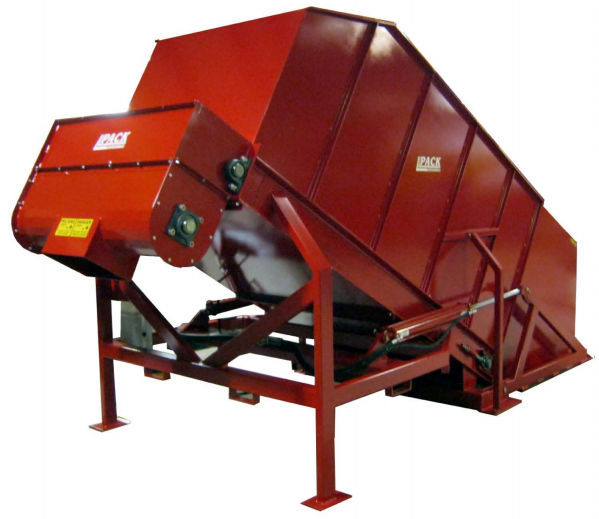
\includegraphics[width=.9\linewidth]{./img_uf1596/big_bale.jpg}
\end{center}
\item \textbf{Mezcladora}
\begin{center}
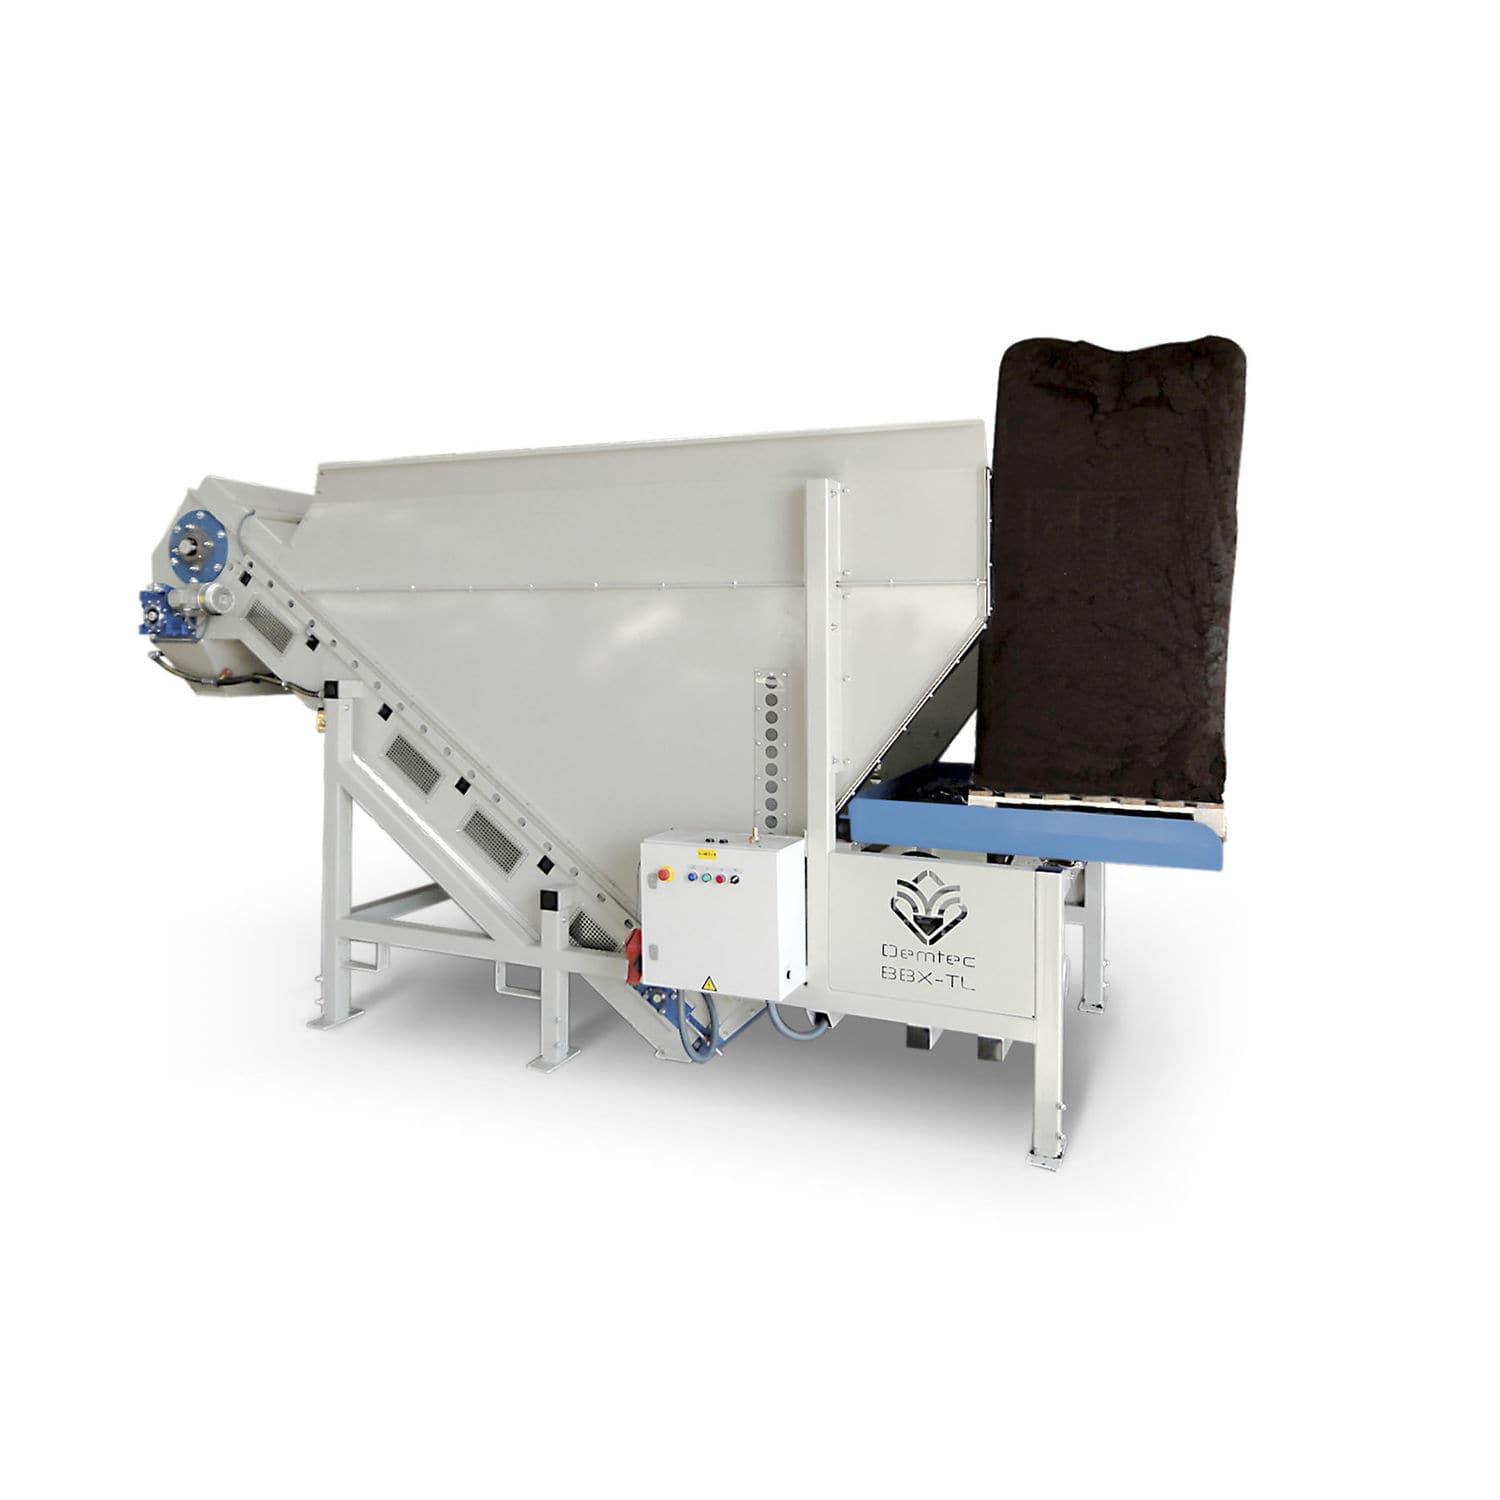
\includegraphics[width=.9\linewidth]{./img_uf1596/mezcladora.jpg}
\end{center}
\item \textbf{Mezcladora y llenadora de bandejas}
\begin{center}
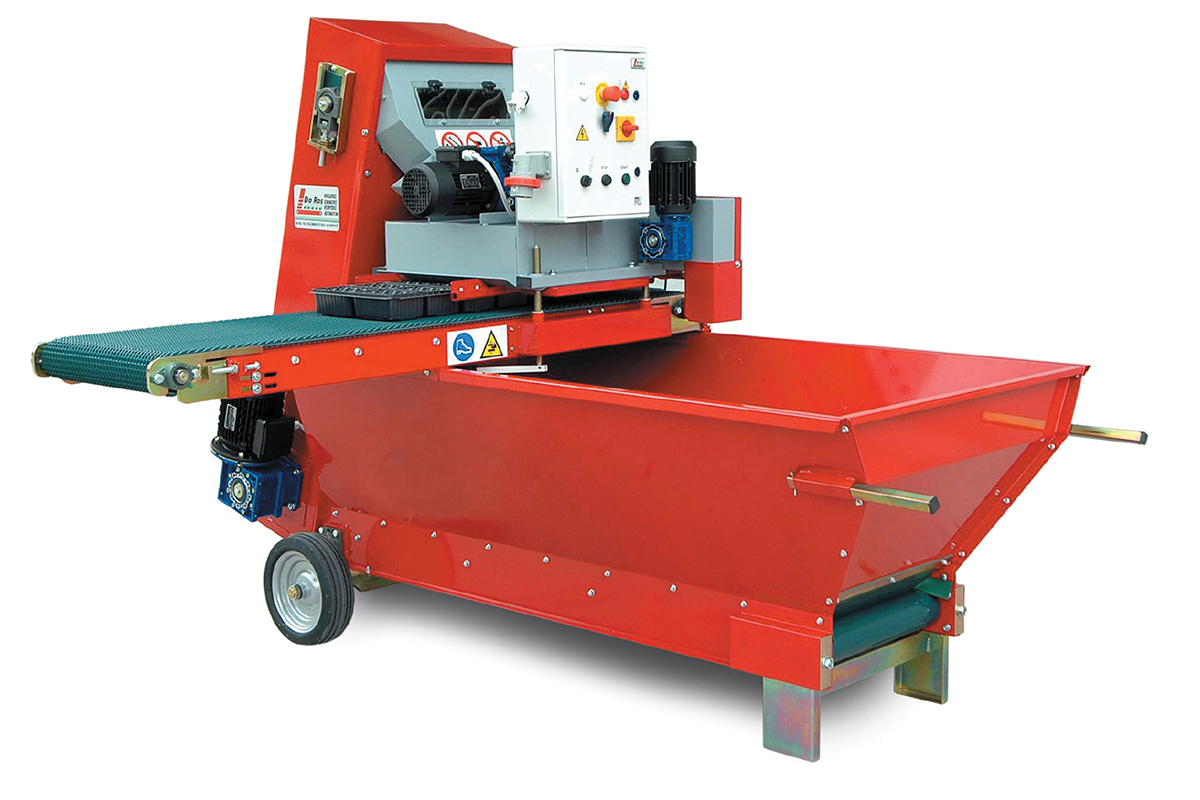
\includegraphics[width=.9\linewidth]{./img_uf1596/bandejas_mezcladora.jpg}
\end{center}
\item \textbf{Enmacetadora}
\begin{center}
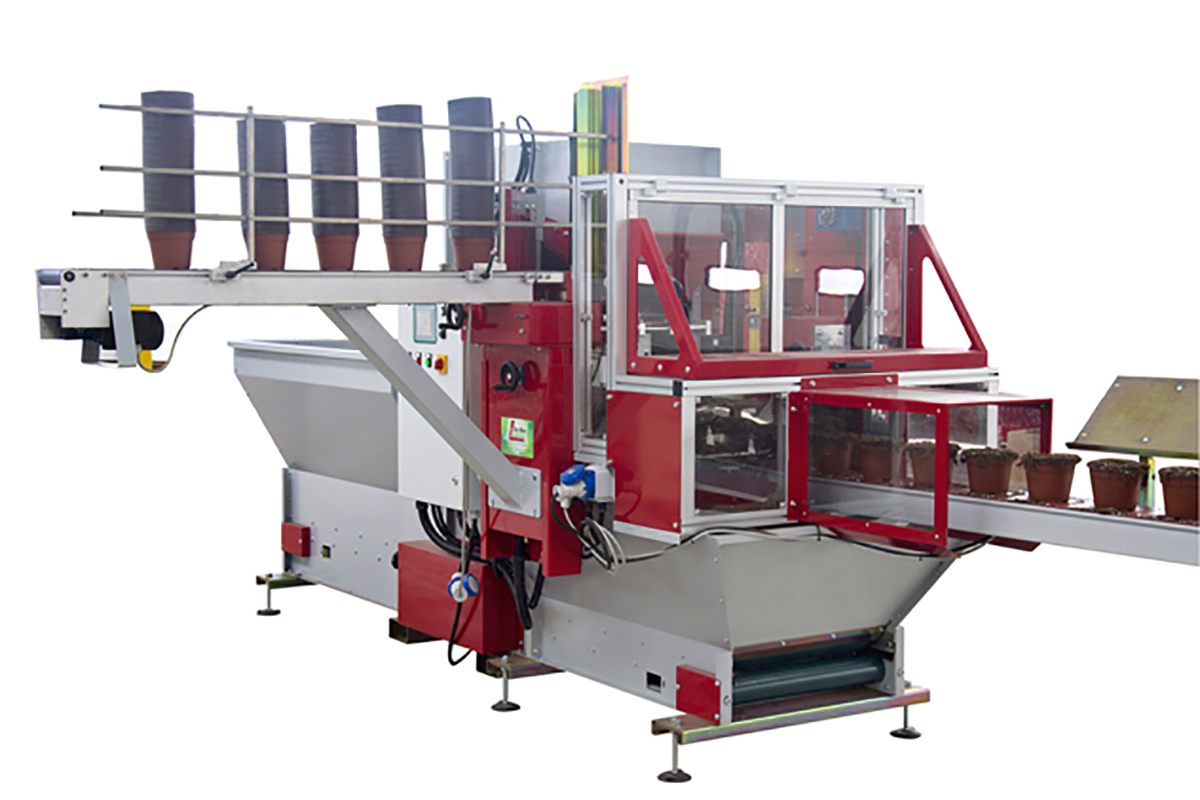
\includegraphics[width=.9\linewidth]{./img_uf1596/enmacetadora.jpg}
\end{center}
\item \textbf{Transplantadora de bandejas}
\begin{center}
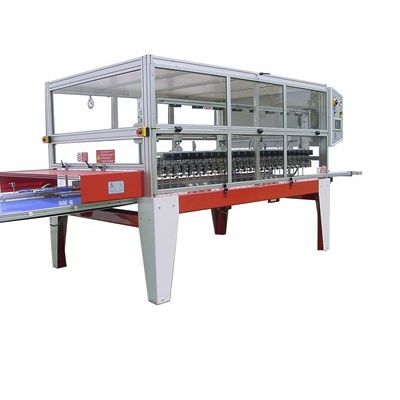
\includegraphics[width=.9\linewidth]{./img_uf1596/transplantadora_bandejas.jpg}
\end{center}
\item \textbf{Sembradora de líneas}
\begin{center}
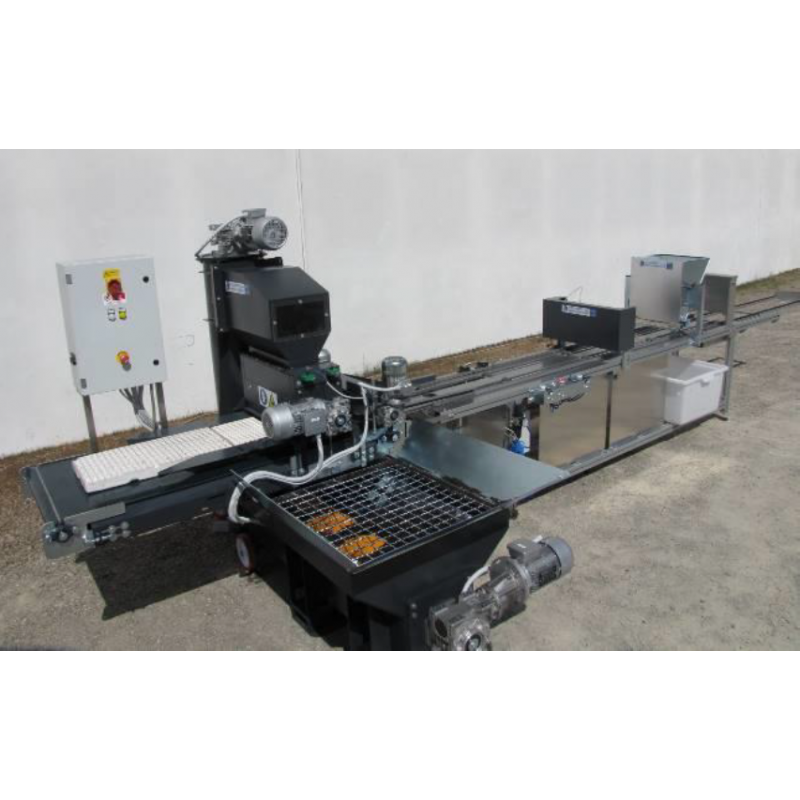
\includegraphics[width=.9\linewidth]{./img_uf1596/sembradora_bandejas.png}
\end{center}
\end{itemize}
\section{Técnicas de transplante}
\label{sec:org5d33378}
\subsection{Introducción}
\label{sec:org421459f}
El transplante consiste en trasladar una planta de una maceta a otra más grande
o al terreno definitivo.

Para realizar el transplante hay que \uline{tener en cuenta muchos factores}, por lo
que \uline{no se pueden} dar unas pautas fijas de cuando y como. Pero \uline{si se puede}
dar \textbf{una norma clara y concisa}:
\begin{center}
\textbf{"El transplante se realiza cuando la planta ha llenado con raices todo el
 contenedor. Idealmente "} 
\end{center}
\subsection{Estadios de desarrollo del cultivo}
\label{sec:orgd83cb82}
Las plantas que hay que transplantar pueden proceder de:
\begin{itemize}
\item Multiplicación vegetativa, \uline{generalmente esquejes}. Podemos encontrar los
siguientes \_tipos de esquejes:
\begin{itemize}
\item Esquejes herbáceos: clavel, crisantemo, salvia
\item Esquejes de madera blanda o semiverde: Aquellos tallos que no han comenzado
a lignificarse.
\item Esquejes de madera semidura: el tallo ha comenzado el proceso de
lignificación pero no es leñoso del todo. Se emplea para especies arbustivas
sobre todo
\begin{itemize}
\item Boj (Buxus sempervirens)
\item Callistemon (Callistemon rigidus)
\item Adelfa (Nerium olenader)
\item Pitosporo (Pittosporum tobira)
\end{itemize}
\item Esquejes de madera dura de especies perennes
\begin{itemize}
\item Árbol de Júpiter (Lagerstroemia indica)
\item Hibisco (Hibiscus siryacus)
\item Rosal (Rosa spp.)
\end{itemize}
\item Especies de madera dura de especies caducas
\begin{itemize}
\item Higuera (Ficus carica)
\item Chopo (Popoulus spp.)
\item Ginkgo (Ginkgo biloba)
\item Agracejo (Berberis spp.)
\end{itemize}
\end{itemize}
\item Multiplicación por semillas o sexual
\end{itemize}

El \uline{enraizamiento} de los esquejes se inicia en unas condiciones optimas de
\uline{humedad y temperatura}. Consideramos que está suficientemente desarrollado
cuando se puede extraer con el esqueje \uline{todo el cepellón} con facilidad.

Las plantas que proceden de semilla \uline{estarán preparadas} para el tranplante al
igual que los esquejes, cuando las raices se han desarrollado \uline{suficientemente}
por odo el alveolo y podemos extraer el cepellón con facilidad. 

\uline{El tiempo} que debe transcurrir para la \uline{germinación} varía mucho de unas
especies a otras. Cambia en función de \uline{condiciones de cultivo} como son
\uline{temperatura, luminosidad, medio de cultivo, humedad ambiental}, etc
\subsection{Operaciones pre-transplante.}
\label{sec:orgef7362e}
\subsubsection{Endurecimiento}
\label{sec:orgd89021a}
Consiste en someter a las plántulas a una serie de \uline{condiciones ambientales
adversas} para que resistan  mejor el tranplante.

Con el  endurecimiento conseguimos que la planta \uline{detenga o disminuya el
crecimiento de la parte aérea} y de esta manera favorecemos que \uline{se desarrolle
el sistema radicular}, y la acumulación de sustancias de reserva. 

Podemos conseguir el endurecimiento de tres formas:
\begin{itemize}
\item Por bajas temperaturas
\item Por estrés hidrico
\item Por falta de determinados nutrientes como nitrogeno (N) y potasio (K)
\end{itemize}

Cuando se realiza el endurecimieto \uline{hay que tener muy cen cuenta} las
condiciones en las que están las plantas y las condiciones que tendrán que
soportar en el tranplante
\subsubsection{Recepción del material}
\label{sec:orgbbbf97e}
Puede que las plantas las hayamos producido nosotros o vengan de otro
viviero. En cualquier caso \uline{hay que prestar atención al estado en que nos
llegan} antes de proceder a su transplante.
\begin{enumerate}
\item \textbf{Algunas recomendaciones para el descarte de plantas:}
\begin{itemize}
\item En primer lugar descartaremos las que tengan \uline{signos de enfermedades o ataques}
de plagas, las debiles, las que tengan heridas y las deformes.
\item Las plantas \uline{vivaces} han de tener buen aspecto. Descartaremos las raquiticas
o envejecidas, con tallo pelado y las que tengan flores \uline{solo en su parte más
alta}
\end{itemize}
\item \textbf{Recomendaciones para la revisión general de plantas:}
\begin{itemize}
\item \uline{Regar los semilleros} para poder extraer facilmente el cepellón \uline{sin dañar
las raices}
\item Transplantar las que tengan un aspecto \uline{sano, con hojas bien desarrolladas
y buen color}
\item Las plantas \uline{deben tener} un sistema radicular \uline{bien desarrollado}, con
raices \uline{blancas y delgadas}. La presencia de \uline{raices marrones} son señal de
exceso de humedad o problemas de pudriciones radicales
\end{itemize}
\end{enumerate}
\subsection{Tipos de contenedores}
\label{sec:orgdd5396e}
Los contenedores son muy importantes ya que son el suelo de las
plantas. Cualquier recipiente puede ser utilizado como maceta para mantener una
planta, pero para a \uline{producción de planta los contenedores deben satisfacer
otras necesidades}.
\subsubsection{Cualidades de los contenedores para producción de planta}
\label{sec:org0dac310}
\begin{itemize}
\item Ante todo ser \textbf{funcional} y permitir la \textbf{mecanización} (llenado y semillado
por ejemplo)
\item \textbf{Manejable} y \textbf{Resistente}
\item Ocupar mínimo \textbf{espacio}
\item Que se pueda \textbf{agrupar} en bandejas y/o apilar
\item Que se pueda reciclar (utilizar varias veces)
\end{itemize}
\subsubsection{Materiales}
\label{sec:org0129e9e}
A continuación describimos los principales materiales empleados en la
fabricación de contenedores para producción de planta.
\begin{enumerate}
\item Macetas biodegradables
\label{sec:org296b6ac}
\end{enumerate}
\end{document}